\section{引言}
现有 TSAD 基准衡量异常分数能否预测异常，却不衡量它是否在时间序列已有的简单统计信号之外贡献信息。这是两个不同问题。局部方差和偏差本身就可以成为有竞争力的异常分数~\cite{zhu2026oneliners}；现代检测器可能得分很高却主要复现这些信号，而排名较低的检测器也可能提供互补异常证据。TSB-AD 等基准~\cite{liu2024tsbad} 揭示独立表现，却没有揭示新增贡献。

这引出两个不同问题。第一，统计参考 $B$ 能在多大程度上重构检测器分数 $S_D$？第二，给定 $B$ 后，$S_D$ 还能提供多少新增标签预测效用？前者衡量统计重合，后者衡量检测器是否在这种重合之外提供异常证据。仅有差异不足以证明有用：独立噪声也能与参考不同，却不改善预测。

我们提出条件检测效用（CDU），补上当前 TSAD 基准缺失的评价维度。CDU 在保留相同统计参考时，比较加入检测器分数前后的留出对数损失。它与精确率--召回率曲面下体积（VUS-PR）~\cite{paparrizos2022vus} 互补：独立评价问“分数能否预测异常”，条件评价问“它在参考之外增加了什么”。POLY 与 MOMENT-ZS 的 VUS-PR 几乎相同（0.389 对 0.383），但在主要 spline 评价下，POLY 的 CDU 高出 0.00593 比特。检测器独立效用与 CDU 使用相同对数损失时，这一区别依然存在。MOMENT-ZS 又可被统计参考高度重构（$R^2=0.904$），说明统计重合与新增标签效用并非同一概念。

本文有三项贡献。第一，我们指出标准 TSAD 评价的盲点：独立表现无法区分统计冗余与互补标签信号。第二，我们提出 CDU，用来源留出的配对预测评价衡量固定检测器分数在统计参考之外增加的预测价值；其不受限总体对应量是条件互信息。第三，我们在 350 条序列和九个检测器上表明，条件化改变检测器比较，统计可重构性不能决定新增标签效用，而所得到的领先组结构在探针、抽样种子和参考变体下保持稳定。

\section{相关工作}
预测 $\mathcal V$-信息刻画所选预测函数族能够读取的信息~\cite{xu2020usable}；条件探针衡量基线表示之外的信息~\cite{hewitt2021conditional}；预测变量重要性则比较包含与不包含特征时的风险~\cite{williamson2023importance}。我们为异构 TSAD 分数建立共同分数接口、来源留出拟合、匹配的独立/条件损失和来源均衡汇总，将这一原则具体化。

TSAD 中的单行统计评分器比较揭示了基准表现的重合~\cite{zhu2026oneliners}。时间序列基础模型研究也考察了漂移条件下预测误差特征在窗口统计量之外的价值~\cite{stability2026}。本文聚焦于跨检测器家族的共同分数级条件评价，采用匹配损失和来源留出测试。

\section{条件检测效用}
\subsection{配对预测评价}
令 $Y\in\{0,1\}$ 为异常标签，$B\in\mathbb R^p$ 为统计参考，$S_D$ 为检测器分数。对每个留出来源，从相同探针族 $\Probe$ 拟合两个概率预测器：一个接收 $B$，另一个接收 $(B,S_D)$。二者使用相同训练点、权重和拟合设置。实际估计为
\begin{equation}
\widehat{\CDU}_{\Probe}(D\mid B)=\widehat L_B-\widehat L_{BD},
\label{eq:cdu}
\end{equation}
其中 $\widehat L_B$、$\widehat L_{BD}$ 是以比特计量的配对留出对数损失。CDU 为正表示给定参考后，检测器改善了标签预测。图~\ref{fig:protocol} 概括了这一比较。

匹配的独立效用定义为 $U_D=\widehat L_0-\widehat L_D$。检测器独立探针仅接收 $S_D$，空模型则预测仅从训练来源估计的加权异常先验。因此 $U_D$ 与 CDU 使用相同损失，但参考信息不同。

\subsection{总体解释}
定义 $\Risk^*(X)=\inf_q\E[-\log_2 q(Y\mid X)]$，其中 $q$ 遍历条件概率分布。
\par\noindent\textbf{命题 1。} 在共同联合分布下，对于不受限预测器，
\begin{equation}
\begin{aligned}
\CDU^*(D\mid B)&=\Risk^*(B)-\Risk^*(B,S_D)\\
&=I(Y;S_D\mid B).
\end{aligned}
\end{equation}
\noindent\textit{证明。} 交叉熵分解给出
\begin{equation}
\begin{aligned}
\E[-\log_2 q(Y\mid X)]&=H(Y\mid X)\\
&\quad+\E_X[D_{\rm KL}(P_{Y\mid X}\Vert q_{Y\mid X})].
\end{aligned}
\end{equation}
KL 项非负且在 $q=P$ 时为零，所以 $\Risk^*(X)=H(Y\mid X)$。两项条件熵相减即得结论。\hfill$\square$

因此总体 CDU 非负，且 $S_D=g(B)$ 时为零：完全由参考决定的分数不增加信息。有限探针 CDU 是相对于预测函数族的新增预测效用可操作估计；有限样本跨来源迁移时，拟合估计可以为负。

\subsection{共同分数表示}
每条分数曲线与标签采用相同时间索引。我们用序列内平均秩评价异常排序信息，并移除检测器特有的分数间距。对长度为 $T_i$ 的曲线，秩从一开始计数：
\begin{equation}
\widetilde s_{it}=\frac{\operatorname{rank}_{\rm avg}(s_{it})-0.5}{T_i}.
\end{equation}
统计参考采用相同排名表示。并列关系保留，常数曲线映射为 0.5。秩归一化是评价定义的一部分：它衡量检测器异常排序在秩归一化统计参考之外新增的标签信息。该变换不使用标签；下文 $B$ 与 $S_D$ 指这些探针输入。

\subsection{留一来源探针评价}
来源指基准的数据集分组。每个外层折从探针训练中排除某一来源的全部序列，其余来源的标签监督探针；留出标签仅用于计算损失。检测器输出与统计参考保持固定。这一严格拆分阻止探针利用留出来源的同源序列。

令 $G_{\rm tr}$ 为训练来源数，$n_g$ 为来源 $g$ 的序列数。若序列 $i$ 保留 $m_i$ 个训练点且 $N_s=\sum_i m_i$，则每个保留点的权重为
\begin{equation}
w_{it}=\frac{N_s}{G_{\rm tr}n_gm_i}.
\end{equation}
各来源总权重相等，来源内各序列总权重相等。全量训练取 $m_i=T_i$，抽样训练取 $m_i=\min(T_i,2048)$，权重之和为 $N_s$。每折共同的基底预测器为全部检测器提供参考损失。

\begin{figure}[t]
\centering
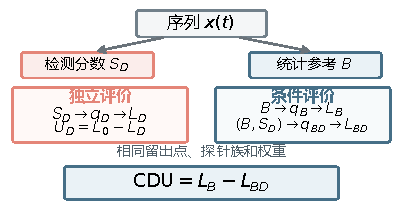
\includegraphics[width=\columnwidth]{figures/protocol_zh.pdf}
\caption{同一序列产生统计参考与检测器分数。独立效用只使用该分数；CDU 比较加入该分数前后的配对探针。}
\label{fig:protocol}
\end{figure}

\subsection{汇总与不确定性}
对于输入设置 $M\in\{0,B,D,BD\}$，令 $p_{it}^{M}$ 为留出异常概率。采用二元对数损失 $\ell(y,p)=-y\log_2p-(1-y)\log_2(1-p)$，计算
\begin{equation}
L_i^M=\frac{1}{T_i}\sum_{t=1}^{T_i}\ell(y_{it},p_{it}^{M}).
\end{equation}
所有测试点均保留。先在来源内平均，再对 $G_{\rm all}$ 个来源等权平均：
\begin{equation}
L_g^M=\frac{1}{n_g}\sum_{i\in g}L_i^M,\qquad
\widehat L_M=\frac{1}{G_{\rm all}}\sum_g L_g^M.
\end{equation}
本研究 $G_{\rm all}=23$、$G_{\rm tr}=22$。配对来源 Bootstrap 95\% 区间刻画给定外层折拟合探针后的留出来源变异。

\input{tables/primary_results_zh}
\begin{figure*}[!t]
\centering
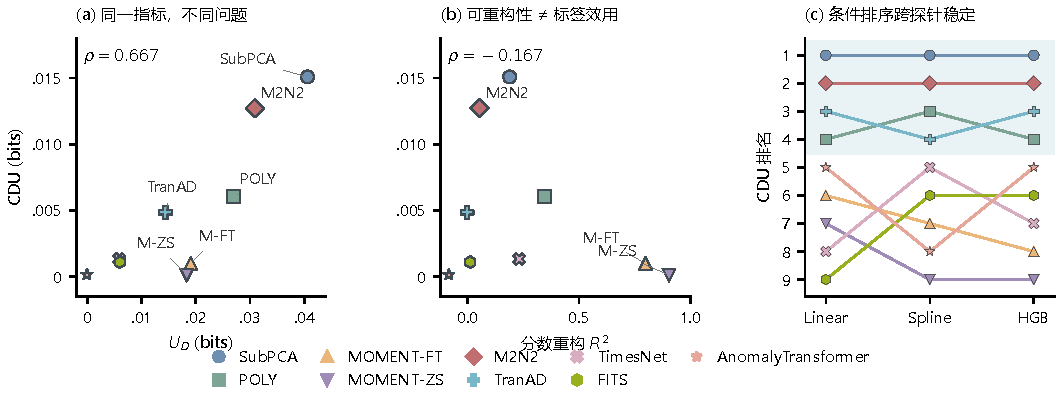
\includegraphics[width=\textwidth]{figures/conditional_comparison_zh.pdf}
\caption{基准盲点及其后果：（a）检测器独立效用与条件效用使用相同 spline 探针和对数损失，结果仍不同；（b）统计可重构性不能决定新增标签效用；（c）条件排序跨探针稳定。前两名次序及阴影所示前四名集合保持不变。}
\label{fig:intervals}
\end{figure*}

\section{实验设置}
\label{sec:setup}
\textbf{数据与检测器。} 我们评价 TSB-AD-U~\cite{liu2024tsbad} 的 350 条单变量序列，采用文献~\cite{zhu2026oneliners} 中的评价样本集合。来源由文件名的数据集标识划分，MSL 与 SMAP 分开，UCR 整个档案归为一组。九个检测器包括基准中的 SubPCA、POLY~\cite{liu2024tsbad}，微调（FT）和零样本（ZS）MOMENT~\cite{goswami2024moment}，M2N2~\cite{kim2024m2n2}、TranAD~\cite{tuli2022tranad}、TimesNet~\cite{wu2023timesnet}、FITS~\cite{xu2024fits} 及 AnomalyTransformer~\cite{xu2022anomaly}。每个检测器均保留全部 350 条曲线。

\textbf{统计参考。} 31 个固定、无标签特征覆盖局部方差、极差、预测偏差、绝对差分、稳健分散度与谱熵。方差与均值偏差由~\cite{zhu2026oneliners} 启发，其余家族扩展参考，并且不使用留出标签选择特征。

\textbf{探针与比较。} 主要探针采用加性三次 spline logistic，linear logistic 与直方图梯度提升（HGB）作为稳健性探针。三者使用相同的均匀、无标签训练抽样（每序列最多 2048 点）、来源/序列权重和完整测试曲线。Logistic 固定逆 L2 正则化强度 $C=0.1$；spline 在 $[0,1]$ 上设四个固定结点，HGB 为 32 次迭代的浅层树集成。不额外进行类别重加权或超参数搜索。VUS-PR 与 CDU 使用相同检测器曲线。

\textbf{分数重构与稳健性。} 来源留出的 ridge 回归用秩化的 31 维统计参考预测各检测器的秩化分数（$\alpha=1$）；训练每序列最多抽样 2048 点，留出曲线使用全部时间点。报告来源宏平均 $R^2$ 与 Spearman 相关性。稳健性分析在保持秩化参考不变的情况下，重复五个训练抽样种子、七种删除单一特征家族及累积 7--29 维参考，并改变检测器分数接口。替代接口分别采用序列内最小--最大缩放，以及序列内 z-score 的高斯累积分布函数。

\textbf{对照。} 对照包括复制参考特征、独立标准正态噪声，以及对 $Z+2Y$（独立 $Z\sim\mathcal N(0,1)$）做秩变换的合成分数，分别代表冗余、无关和新增标签信号。仅合成对照使用标签。

\section{结果与解释}
\subsection{独立表现与新增效用讲述不同故事}
表~\ref{tab:main} 和图~\ref{fig:intervals}a 在相同 spline 探针、对数损失、留出来源和权重下比较检测器独立效用 $U_D$ 与 CDU。MOMENT-FT、MOMENT-ZS 从 $U_D$ 第 4、5 名降至 CDU 第 7、9 名，TranAD 则从第 6 升至第 4。Linear、spline、HGB 下，$U_D$/CDU 排名相关性分别为 0.967、0.667、0.500。基准 VUS-PR 也呈现这种区别：M2N2、TranAD 从 VUS 第 5、6 名变为 CDU 第 2、4 名。

POLY 与两种 MOMENT 的 VUS-PR 接近（0.3832--0.3893），但 POLY 的 spline CDU 比 MOMENT-FT 高 0.00505 比特 [0.00172, 0.00860]，比 MOMENT-ZS 高 0.00593 [0.00241, 0.00961]。三种探针共九项配对比较经最大标准化 Bootstrap 联合校正后，两组区间仍为正。

\subsection{分数可重构性不能决定新增标签效用}
来源留出的 ridge 回归较强地重构 MOMENT-FT 和 MOMENT-ZS 分数（来源宏平均 $R^2=0.799$、0.904；Spearman 为 0.895、0.951），对 M2N2 和 TranAD 则较弱（$R^2=0.054$、$-0.002$）。九模型的重构 $R^2$ 与 spline CDU 的 Spearman 相关性为 $-0.167$（图~\ref{fig:intervals}b）。在这九个检测器中，统计重合与新增标签效用对应较弱：难以重构的分数只有在残余信息改善标签预测时才有价值。

\subsection{条件比较具有可重复性}
Linear、spline 和 HGB 下，SubPCA 与 M2N2 始终排第一、第二，TranAD 与 POLY 组成相同前四名集合（图~\ref{fig:intervals}c）。探针两两排名相关性为 0.717--0.867。Spline 和 HGB 从统计参考中提取的预测信号显著多于 linear logistic：其基底损失分别为 0.2891、0.2869 比特，linear 为 0.3375。线性训练从抽样扩展至全量，基底损失几乎不变（0.337462 对 0.337447），表明差距主要来自探针表达能力，而非训练点数增加。

五个训练抽样种子得到完全相同的 spline 排名。七组参考家族删除的排名相关性为 0.917--1.000；含 7--29 个特征的累积参考保留完整参考的前四名（$\rho=0.933$--1.000）。检测器分数经序列内 z-score 与高斯累积分布函数变换后也保留该领先组（$\rho=0.933$）。最小--最大缩放保留检测器特有的原始分数间距，改变更广泛的排名（$\rho=0.517$），使 POLY 从第 3 降至第 9。这一对照说明采用共同秩接口的理由：主要 CDU 比较衡量异常排序信息，而非检测器特有的分数几何结构。

\subsection{对照验证预期行为}
匹配复制与独立噪声对照均接近零，没有负向对照的区间完全高于零。所有标签相关合成对照明显为正；spline 合成 CDU 为 0.09220 比特 [0.06819, 0.11712]。CDU 区分冗余、无关和互补的标签信号。


\section{讨论与结论}
TSAD 基准衡量异常对应关系；CDU 衡量统计参考之外的新增效用。九模型的匹配损失比较改变排名，分数重构则区分统计重合与新增标签效用。领先组在探针、种子及所测试的参考下保持稳定。

CDU 有意相对于参考和探针定义，不赋予架构因果解释。将它与独立表现共同报告，可以区分当前基准排名混为一谈的两个问题：检测器是否有效，以及它在简单统计结构之外增加了什么。

{\footnotesize\noindent\textbf{致谢。}OpenAI Codex 辅助起草第 1--6 节及评价/绘图代码；最终内容均由作者验证。\par}
